\subsection{Módulo de \textit{input}}

Os estados dos botões do GBA ficam salvos em um registrador. Cada um desses estados é representado por um \textit{bit} no valor guardado por esse registrador. Sempre que um botão é apertado, o GBA automaticamente troca o valor guardado nesse registrador de tal forma que o \textit{bit} que representa o botão em questão passe a possuir valor 0. De forma similar, quando o botão é solto, o valor contido no \textit{bit} em questão é modificado para 1, seu valor padrão. Sendo assim, a checagem dos estados pode ser realizada facilmente utilizando \textit{bitmasks}. Por exemplo, caso se deseje checar um botão representado pelo \textit{bit} 2 (com a contagem começando em 0), basta pegar o resultado do \textit{AND} binário entre o valor guardado no registrador e a potência de 2 que possui como expotente o \textit{bit} em questão (4, nesse exemplo). Abaixo é possível vizualizar no código do módulo de \textit{input} a definição das constantes que representam os botões, assim como a função utilizada para checar o estado de cada um deles:

\begin{minted}[frame=lines, linenos]
{c++}
#ifndef INPUT\_H
#define INPUT\_H

#include <stdbool.h>
#include "base\_types.h"

#define BUTTON\_A 1
#define BUTTON\_B 2
#define BUTTON\_SELECT 4
#define BUTTON\_START 8
#define BUTTON\_RIGHT 16
#define BUTTON\_LEFT 32
#define BUTTON\_UP 64
#define BUTTON\_DOWN 128
#define BUTTON\_R 256
#define BUTTON\_L 512

#define N\_BUTTON 10

int pressed\_state[N\_BUTTON];

void check\_buttons\_states();
bool pressed(int button);

#endif
\end{minted}
\makebox[\linewidth]{Cabeçalho do módulo de input. Fonte: \textit{Autores}.}
\vspace{\onelineskip}

\begin{minted}[frame=lines, linenos]
{c++}
#include "input.h"

volatile unsigned int *buttons_mem = (volatile unsigned int *)0x04000130;

void check_buttons_states() {
    for(int i = 0; i < N_BUTTON; i++) {
        pressed_state[i] = !((*buttons_mem) & (1 << i));
    }
}

bool pressed(int button) {
    return pressed_state[button];
}
\end{minted}
\makebox[\linewidth]{Código fonte do módulo de input. Fonte: \textit{Autores}.}
\vspace{\onelineskip}

Abaixo é possível visualizar um teste implementado para checar o pressionamento dos botões do GBA. Para cada botão pressionado um \textit{pixel} vermelho aparece na tela. Na imagem abaixo, os botões B, R, \textit{LEFT}, \textit{RIGHT} e \textit{START} estão sendo pressionados simultaneamente.

\begin{figure}[H]
 \centering 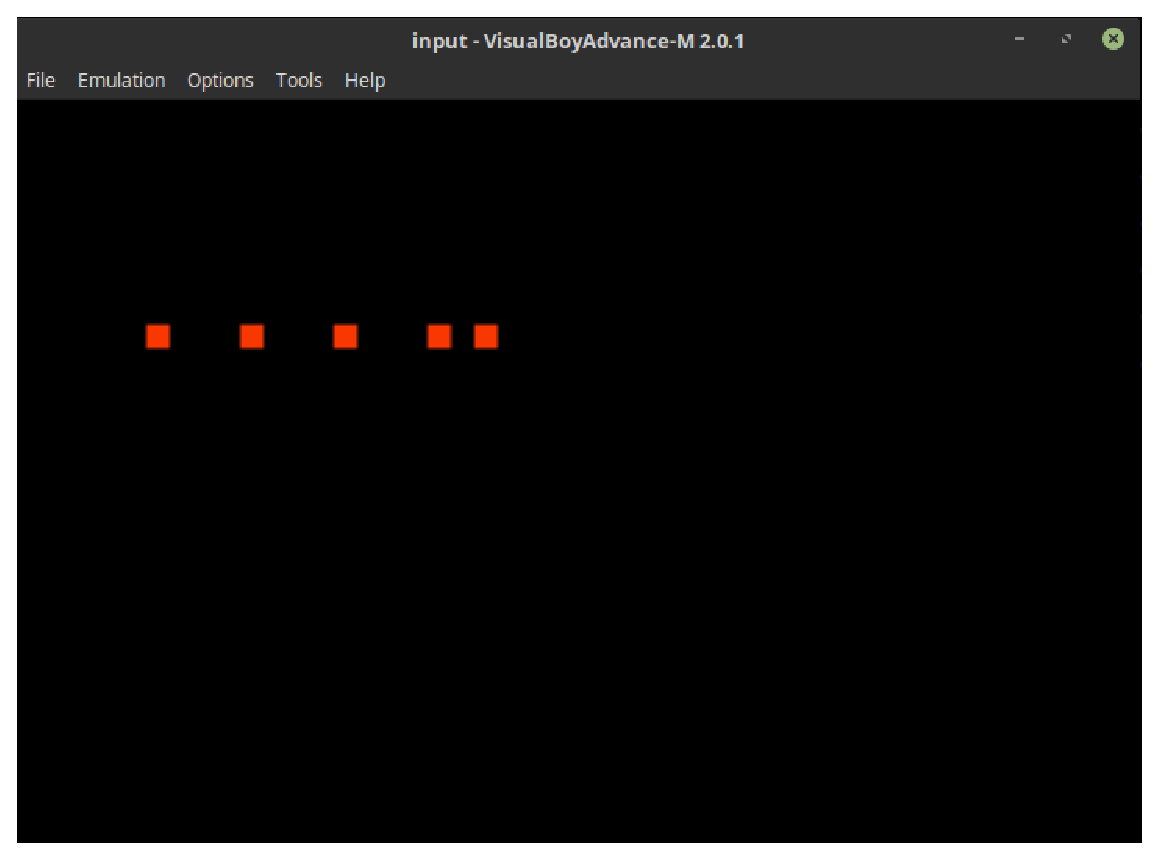
\includegraphics[keepaspectratio=true,scale=0.6]{figuras/demo-input.eps}
   \caption[Demonstração do pressionamento de botões no emulador]
    {Teste de pressionamento de botões no emulador. Fonte: \textit{Autores}.}
   \label{demo-input}
\end{figure}

Abaixo se encontra o código fonte escrito para a realização deste teste:

\begin{minted}[frame=lines, linenos]
{c++}
#include "video.h"
#include "input.h"

#define RED 0x0000FF

unsigned short *vid_mem = (unsigned short *)0x6000000;

int main() {
    reset_dispcnt();
    set_video_mode(3);
    set_background_number(2);

    while(1) {
        check_buttons_states();

        for(int i=0;i<=9;i++){
            if (pressed(i)) {
                vid_mem[50 * 240 + i * 10] = RED;
            } else {
                vid_mem[50 * 240 + i * 10] = 0;
            }
        }
    }

    return 0;
}
\end{minted}
\makebox[\linewidth]{Código fonte do teste de \textit{input}. Fonte: \textit{Autores}.}
\vspace{\onelineskip}